\documentclass{standalone}
\usepackage{tikz}
\usetikzlibrary{patterns, positioning}


\begin{document}
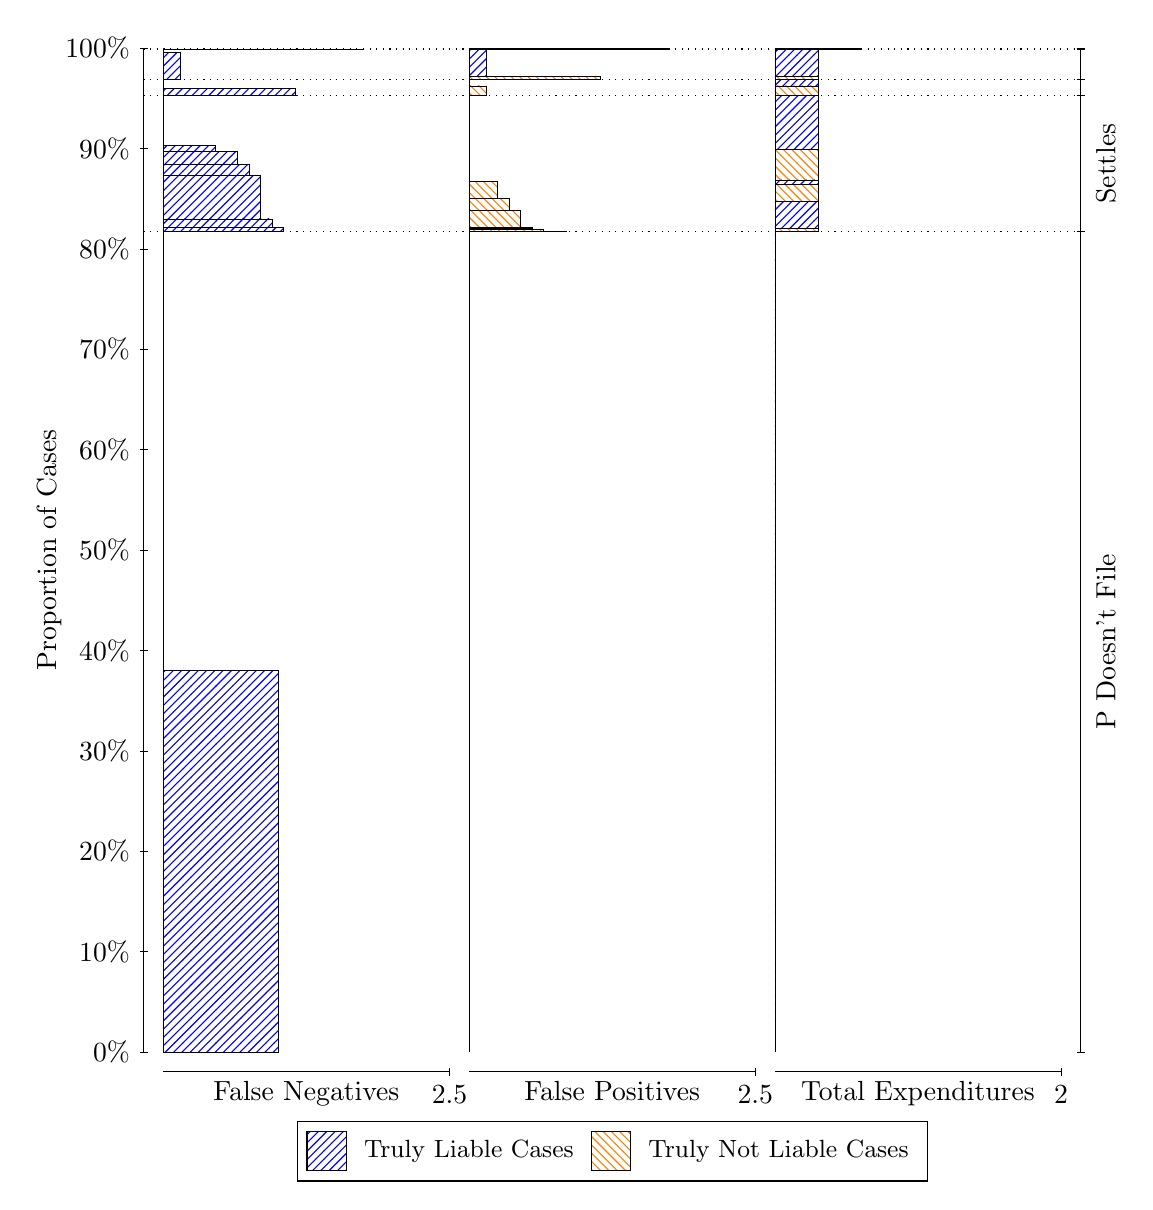
\begin{tikzpicture}
\draw[black, very thin] (1.5,1.75) -- (1.5,14.5);
\node[rotate=90, text=black, anchor=center] at (0.3, 8.125) {Proportion of Cases};
\draw[black, very thin] (1.45,1.75) -- (1.55,1.75);
\node[text=black, anchor=east] at (1.45, 1.75) {0\%};
\draw[black, very thin] (1.45,3.025) -- (1.55,3.025);
\node[text=black, anchor=east] at (1.45, 3.025) {10\%};
\draw[black, very thin] (1.45,4.3) -- (1.55,4.3);
\node[text=black, anchor=east] at (1.45, 4.3) {20\%};
\draw[black, very thin] (1.45,5.575) -- (1.55,5.575);
\node[text=black, anchor=east] at (1.45, 5.575) {30\%};
\draw[black, very thin] (1.45,6.85) -- (1.55,6.85);
\node[text=black, anchor=east] at (1.45, 6.85) {40\%};
\draw[black, very thin] (1.45,8.125) -- (1.55,8.125);
\node[text=black, anchor=east] at (1.45, 8.125) {50\%};
\draw[black, very thin] (1.45,9.4) -- (1.55,9.4);
\node[text=black, anchor=east] at (1.45, 9.4) {60\%};
\draw[black, very thin] (1.45,10.675) -- (1.55,10.675);
\node[text=black, anchor=east] at (1.45, 10.675) {70\%};
\draw[black, very thin] (1.45,11.95) -- (1.55,11.95);
\node[text=black, anchor=east] at (1.45, 11.95) {80\%};
\draw[black, very thin] (1.45,13.225) -- (1.55,13.225);
\node[text=black, anchor=east] at (1.45, 13.225) {90\%};
\draw[black, very thin] (1.45,14.5) -- (1.55,14.5);
\node[text=black, anchor=east] at (1.45, 14.5) {100\%};

\draw[black, very thin] (13.4,1.75) -- (13.4,14.5);
\draw[black, very thin] (13.35,1.75) -- (13.45,1.75);
\node[anchor=west] at (13.35, 1.75) {};
\draw[black, very thin] (13.35,12.169) -- (13.45,12.169);
\node[anchor=west] at (13.35, 12.169) {};
\draw[black, very thin] (13.35,13.902) -- (13.45,13.902);
\node[anchor=west] at (13.35, 13.902) {};
\draw[black, very thin] (13.35,14.103) -- (13.45,14.103);
\node[anchor=west] at (13.35, 14.103) {};
\draw[black, very thin] (13.35,14.484) -- (13.45,14.484);
\node[anchor=west] at (13.35, 14.484) {};
\draw[black, very thin] (13.35,14.489) -- (13.45,14.489);
\node[anchor=west] at (13.35, 14.489) {};
\draw[black, very thin] (13.35,14.5) -- (13.45,14.5);
\node[anchor=west] at (13.35, 14.5) {};

\draw[black, very thin, pattern color=blue, pattern=north east lines] (1.75,1.75) rectangle (3.2033,6.5921);
\draw[black, very thin, pattern color=orange, pattern=north west lines] (1.75,6.5921) rectangle (1.75,12.169);
\draw[black, very thin, pattern color=blue, pattern=north east lines] (1.75,12.169) rectangle (3.276,12.226);
\draw[black, very thin, pattern color=blue, pattern=north east lines] (1.75,12.226) rectangle (3.1307,12.331);
\draw[black, very thin, pattern color=blue, pattern=north east lines] (1.75,12.331) rectangle (2.9853,12.88);
\draw[black, very thin, pattern color=blue, pattern=north east lines] (1.75,12.88) rectangle (2.84,13.023);
\draw[black, very thin, pattern color=blue, pattern=north east lines] (1.75,13.023) rectangle (2.6947,13.191);
\draw[black, very thin, pattern color=blue, pattern=north east lines] (1.75,13.191) rectangle (2.404,13.263);
\draw[black, very thin, pattern color=orange, pattern=north west lines] (1.75,13.263) rectangle (1.75,13.902);
\draw[black, very thin, pattern color=blue, pattern=north east lines] (1.75,13.902) rectangle (3.4213,13.988);
\draw[black, very thin, pattern color=orange, pattern=north west lines] (1.75,13.988) rectangle (1.75,14.103);
\draw[black, very thin, pattern color=blue, pattern=north east lines] (1.75,14.103) rectangle (1.968,14.445);
\draw[black, very thin, pattern color=orange, pattern=north west lines] (1.75,14.445) rectangle (1.75,14.484);
\draw[black, very thin, pattern color=blue, pattern=north east lines] (1.75,14.484) rectangle (4.2933,14.487);
\draw[black, very thin, pattern color=orange, pattern=north west lines] (1.75,14.487) rectangle (1.75,14.489);
\draw[black, very thin, pattern color=orange, pattern=north west lines] (1.75,14.489) rectangle (1.75,14.492);
\draw[black, very thin, pattern color=blue, pattern=north east lines] (1.75,14.492) rectangle (1.75,14.5);
\draw[black, very thin, pattern color=orange, pattern=north west lines] (5.6333,1.75) rectangle (5.6333,7.3266);
\draw[black, very thin, pattern color=blue, pattern=north east lines] (5.6333,7.3266) rectangle (5.6333,12.169);
\draw[black, very thin, pattern color=orange, pattern=north west lines] (5.6333,12.169) rectangle (6.8687,12.175);
\draw[black, very thin, pattern color=orange, pattern=north west lines] (5.6333,12.175) rectangle (6.578,12.194);
\draw[black, very thin, pattern color=orange, pattern=north west lines] (5.6333,12.194) rectangle (6.4327,12.208);
\draw[black, very thin, pattern color=orange, pattern=north west lines] (5.6333,12.208) rectangle (6.4327,12.221);
\draw[black, very thin, pattern color=orange, pattern=north west lines] (5.6333,12.221) rectangle (6.2873,12.44);
\draw[black, very thin, pattern color=orange, pattern=north west lines] (5.6333,12.44) rectangle (6.142,12.593);
\draw[black, very thin, pattern color=orange, pattern=north west lines] (5.6333,12.593) rectangle (5.9967,12.808);
\draw[black, very thin, pattern color=blue, pattern=north east lines] (5.6333,12.808) rectangle (5.6333,13.902);
\draw[black, very thin, pattern color=orange, pattern=north west lines] (5.6333,13.902) rectangle (5.8513,14.018);
\draw[black, very thin, pattern color=blue, pattern=north east lines] (5.6333,14.018) rectangle (5.6333,14.103);
\draw[black, very thin, pattern color=orange, pattern=north west lines] (5.6333,14.103) rectangle (7.3047,14.142);
\draw[black, very thin, pattern color=blue, pattern=north east lines] (5.6333,14.142) rectangle (5.8513,14.484);
\draw[black, very thin, pattern color=orange, pattern=north west lines] (5.6333,14.484) rectangle (5.6333,14.487);
\draw[black, very thin, pattern color=blue, pattern=north east lines] (5.6333,14.487) rectangle (5.6333,14.489);
\draw[black, very thin, pattern color=orange, pattern=north west lines] (5.6333,14.489) rectangle (8.1767,14.492);
\draw[black, very thin, pattern color=blue, pattern=north east lines] (5.6333,14.492) rectangle (6.7233,14.5);
\draw[black, very thin, pattern color=orange, pattern=north west lines] (9.5167,1.75) rectangle (9.5167,7.3266);
\draw[black, very thin, pattern color=blue, pattern=north east lines] (9.5167,7.3266) rectangle (9.5167,12.169);
\draw[black, very thin, pattern color=orange, pattern=north west lines] (9.5167,12.169) rectangle (10.062,12.208);
\draw[black, very thin, pattern color=blue, pattern=north east lines] (9.5167,12.208) rectangle (10.062,12.551);
\draw[black, very thin, pattern color=orange, pattern=north west lines] (9.5167,12.551) rectangle (10.062,12.767);
\draw[black, very thin, pattern color=blue, pattern=north east lines] (9.5167,12.767) rectangle (10.062,12.824);
\draw[black, very thin, pattern color=orange, pattern=north west lines] (9.5167,12.824) rectangle (10.062,13.209);
\draw[black, very thin, pattern color=blue, pattern=north east lines] (9.5167,13.209) rectangle (10.062,13.902);
\draw[black, very thin, pattern color=orange, pattern=north west lines] (9.5167,13.902) rectangle (10.062,14.018);
\draw[black, very thin, pattern color=blue, pattern=north east lines] (9.5167,14.018) rectangle (10.062,14.103);
\draw[black, very thin, pattern color=orange, pattern=north west lines] (9.5167,14.103) rectangle (10.062,14.142);
\draw[black, very thin, pattern color=blue, pattern=north east lines] (9.5167,14.142) rectangle (10.062,14.484);
\draw[black, very thin, pattern color=orange, pattern=north west lines] (9.5167,14.484) rectangle (10.607,14.487);
\draw[black, very thin, pattern color=blue, pattern=north east lines] (9.5167,14.487) rectangle (10.607,14.489);
\draw[black, very thin, pattern color=orange, pattern=north west lines] (9.5167,14.489) rectangle (10.607,14.492);
\draw[black, very thin, pattern color=blue, pattern=north east lines] (9.5167,14.492) rectangle (10.607,14.5);
\draw[black, dotted] (1.5,12.169) -- (13.4,12.169);
\draw[black, dotted] (1.5,13.902) -- (13.4,13.902);
\draw[black, dotted] (1.5,14.103) -- (13.4,14.103);
\draw[black, dotted] (1.5,14.484) -- (13.4,14.484);
\draw[black, dotted] (1.5,14.489) -- (13.4,14.489);
\draw[black, very thin] (1.75,1.5) -- (5.3833,1.5);
\node[text=black, anchor=north] at (3.5667, 1.5) {False Negatives};
\draw[black, very thin] (5.3833,1.45) -- (5.3833,1.55);
\node[text=black, anchor=north] at (5.3833, 1.45) {2.5};

\draw[black, very thin] (5.6333,1.5) -- (9.2667,1.5);
\node[text=black, anchor=north] at (7.45, 1.5) {False Positives};
\draw[black, very thin] (9.2667,1.45) -- (9.2667,1.55);
\node[text=black, anchor=north] at (9.2667, 1.45) {2.5};

\draw[black, very thin] (9.5167,1.5) -- (13.15,1.5);
\node[text=black, anchor=north] at (11.333, 1.5) {Total Expenditures};
\draw[black, very thin] (13.15,1.45) -- (13.15,1.55);
\node[text=black, anchor=north] at (13.15, 1.45) {2};

\node[text=black, centered, rotate=90] at (13.72, 6.9593) {P Doesn't File};
\node[text=black, centered, rotate=90] at (13.72, 13.035) {Settles};





\draw (7.449999999999999,1.5) node[draw=none] (baseCoordinate) {};
\begin{scope}[align=center]
        \matrix[scale=0.5, draw=black, below=0.5cm of baseCoordinate, nodes={draw}, column sep=0.1cm]{
            \node[rectangle, draw, minimum width=0.5cm, minimum height=0.5cm, pattern color=blue, pattern=north east lines] {}; &
            \node[draw=none, font=\small, text=black] (B) {Truly Liable Cases}; &
            \node[rectangle, draw, minimum width=0.5cm, minimum height=0.5cm, pattern color=orange, pattern=north west lines] {}; &
            \node[draw=none, font=\small, text=black] (B) {Truly Not Liable Cases}; \\
            };
\end{scope}

\end{tikzpicture}
\end{document}